%%%%%%%%%%%%%%%%%%%%%%%%%%%%%%%%%%%%%%%%%
% Beamer Presentation
% LaTeX Template
% Version 1.0 (10/11/12)
%
% This template has been downloaded from:
% http://www.LaTeXTemplates.com
%
% License:
% CC BY-NC-SA 3.0 (http://creativecommons.org/licenses/by-nc-sa/3.0/)
%
%%%%%%%%%%%%%%%%%%%%%%%%%%%%%%%%%%%%%%%%%

%----------------------------------------------------------------------------------------
%	PACKAGES AND THEMES
%----------------------------------------------------------------------------------------

\documentclass{beamer}

\mode<presentation> {

% The Beamer class comes with a number of default slide themes
% which change the colors and layouts of slides. Below this is a list
% of all the themes, uncomment each in turn to see what they look like.

\usetheme{default}
%\usetheme{AnnArbor}
%\usetheme{Antibes}
%\usetheme{Bergen}
%\usetheme{Berkeley}
%\usetheme{Berlin}
%\usetheme{Boadilla}
%\usetheme{CambridgeUS}
%\usetheme{Copenhagen}
%\usetheme{Darmstadt}
%\usetheme{Dresden}
%\usetheme{Frankfurt}
%\usetheme{Goettingen}
%\usetheme{Hannover}
%\usetheme{Ilmenau}
%\usetheme{JuanLesPins}
%\usetheme{Luebeck}
%\usetheme{Madrid}
%\usetheme{Malmoe}
%\usetheme{Marburg}
%\usetheme{Montpellier}
%\usetheme{PaloAlto}
%\usetheme{Pittsburgh}
%\usetheme{Rochester}
%\usetheme{Singapore}
%\usetheme{Szeged}
%\usetheme{Warsaw}

% As well as themes, the Beamer class has a number of color themes
% for any slide theme. Uncomment each of these in turn to see how it
% changes the colors of your current slide theme.

%\usecolortheme{albatross}
%\usecolortheme{beaver}
%\usecolortheme{beetle}
%\usecolortheme{crane}
%\usecolortheme{dolphin}
%\usecolortheme{dove}
%\usecolortheme{fly}
%\usecolortheme{lily}
%\usecolortheme{orchid}
%\usecolortheme{rose}
%\usecolortheme{seagull}
\usecolortheme{seahorse}
%\usecolortheme{whale}
%\usecolortheme{wolverine}

%\setbeamertemplate{footline} % To remove the footer line in all slides uncomment this line
\setbeamertemplate{footline}[page number] % To replace the footer line in all slides with a simple slide count uncomment this line

\setbeamertemplate{navigation symbols}{} % To remove the navigation symbols from the bottom of all slides uncomment this line
}

%\setbeamertemplate{headline} 

\usepackage{graphicx} % Allows including images
\usepackage{booktabs} % Allows the use of \toprule, \midrule and \bottomrule in tables
\usepackage[export]{adjustbox}
\usepackage{amsmath}
\usepackage[utf8]{inputenc}

%----------------------------------------------------------------------------------------
%	TITLE PAGE
%----------------------------------------------------------------------------------------
%Unfolding the Quantitative Dynamics of Biological Networks
\title[George Christodoulis]{PhD Application Presentation} % The short title appears at the bottom of every slide, the full title is only on the title page

\author{Georgios Christodoulis} % Your name
\institute[NTUA] % Your institution as it will appear on the bottom of every slide, may be shorthand to save space
{
National Technical University of Athens \\ % Your institution for the title page
\medskip
\textit{gchristodoulis@gmail.com} % Your email address
}
\date{\today} % Date, can be changed to a custom date

\begin{document}

\begin{frame}
\titlepage % Print the title page as the first slide
\end{frame}

%%%%%%%%%%%%%%%%%%%%%%%%%%%%%%%%%%%%%%%%%%%%%%%%%%%%%%%%%%%%%%
%			Uncomment for Overview..not for now
%%%%%%%%%%%%%%%%%%%%%%%%%%%%%%%%%%%%%%%%%%%%%%%%%%%%%%%%%%%%%%
%\begin{frame}
%\frametitle{Overview} % Table of contents slide, comment this block out to remove it
%\tableofcontents % Throughout your presentation, if you choose to use \section{} and \subsection{} commands, 
%these will automatically be printed on this slide as an overview of your presentation
%\end{frame}
%%%%%%%%%%%%%%%%%%%%%%%%%%%%%%%%%%%%%%%%%%%%%%%%%%%%%%%%%%%%%%
%----------------------------------------------------------------------------------------
%	PRESENTATION SLIDES
%----------------------------------------------------------------------------------------
%------------------------------------------------
\begin{frame}
\frametitle{Academic Status}
\begin{block}{Diploma (Estim. Graduation: September $2015$)}
Electrical and Computer Engineering School-ECE\\
National Technical University of Athens-NTUA\\
\begin{tabular}{l p{200pt}}
Thesis:&"Performance modeling and Prediction for the communication of parallel applications"
\end{tabular}
\end{block}

\begin{block}{Internship (Until July $17^{th}$ $2015$)}
Laboratoire Spécification et Vérification-LSV\\
Ecole Normale Supérieure de Cachan\\
\begin{tabular}{l p{200pt}}
Topic:&"Petri-net Unfolding of Biological Networks"
\end{tabular}
\end{block}
\end{frame}

%------------------------------------------------
\begin{frame}
\frametitle{Past: High Performance Computing}
\begin{columns}[c]

\column{.8\textwidth}

\begin{block}{Modern Super-Computer Specs}
\begin{enumerate}
\item $\sim30.000$ $8$-core Nodes\\
\item $\sim10$PB Storage / $\sim1000TiB$ Memory\\
\item $\sim30$PFLOPS ($\approx 10^{15}$FLOPS)
\end{enumerate}
\end{block}

\begin{block}{Objectives}
\begin{enumerate}
\item Optimal aplication scaling (linear if possible)
\item Efficient placement and performance prediction
\end{enumerate}
\end{block}

\begin{block}{Challenges}
\begin{enumerate}
\item Exaustive memory interaction
\item Low $\frac{Computation\_load}{Communication\_load}$
\item Vast communication congestion
\end{enumerate}
\end{block}


\column{.2\textwidth}
\begin{figure}
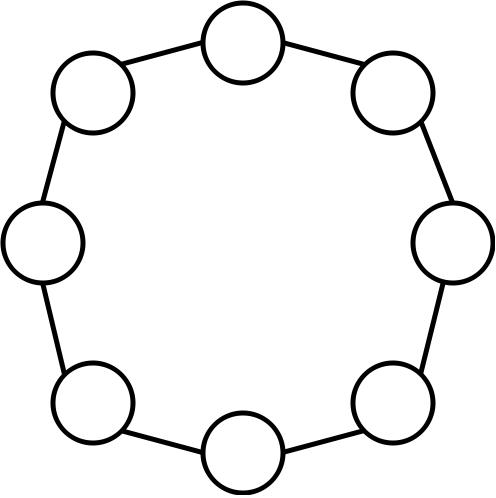
\includegraphics[width=.8\linewidth,right]{ring.jpg}
\end{figure}

\begin{figure}
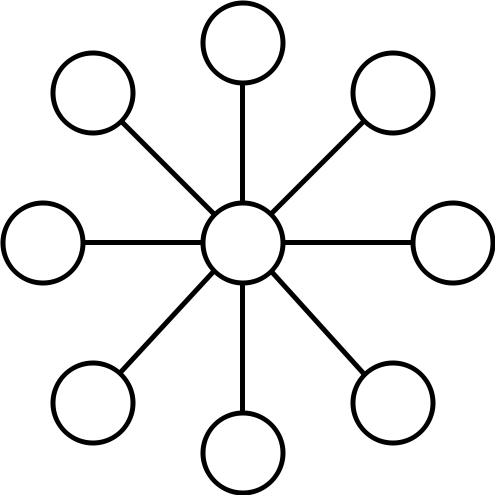
\includegraphics[width=.8\linewidth,right]{star.jpg}
\end{figure}

\begin{figure}
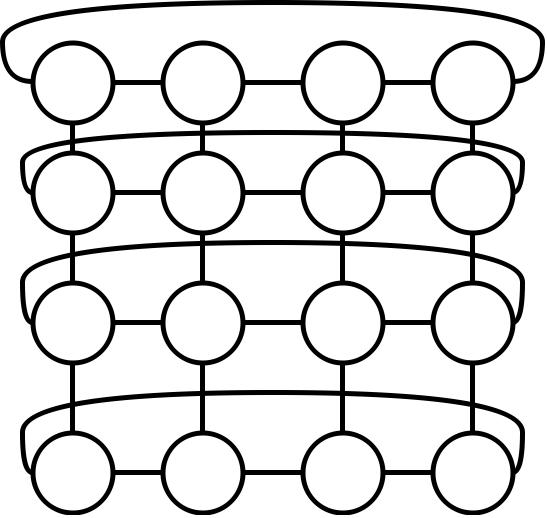
\includegraphics[width=.8\linewidth,right]{torus.jpg}
\end{figure}
\end{columns}
\end{frame}

%------------------------------------------------
\begin{frame}
\frametitle{Biological Challenge}


\begin{columns}[c]

\column{.4\textwidth}
\begin{figure}
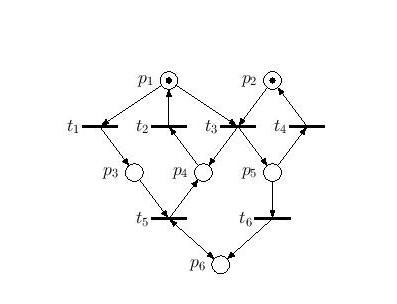
\includegraphics[width=\linewidth,height=\textheight,keepaspectratio]{loic_PN.jpg}
\caption{Petri Net.}
\end{figure}

\column{.4\textwidth}
\begin{figure}
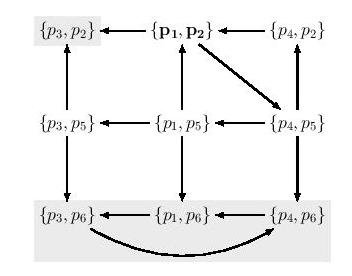
\includegraphics[width=\linewidth,height=\textheight,keepaspectratio]{transition_graph.jpg}
\caption{Equivalent Marking Graph.}
\end{figure}

\column{.3\textwidth}
\begin{figure}
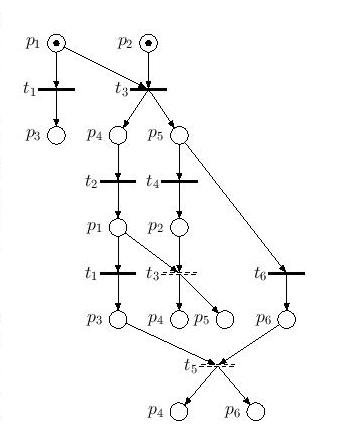
\includegraphics[width=1.1\linewidth,height=\textheight,keepaspectratio]{loic_unfolding.jpg}
\caption{Equivalent Unfolding.}
\end{figure}

\end{columns}
\end{frame}

%------------------------------------------------
\begin{frame}

\end{frame}

%------------------------------------------------
\begin{frame}
\frametitle{Petri-Net Unfolding}
\begin{columns}[c]

\column{.8\textwidth}
\begin{block}{The Unfolding of the network}
\begin{enumerate}
\item Contains the entire information of the system\\
\item Depicts systems' concurrency in a profound and manageable way\\
\item Inherits the properties of partial orders\\
\end{enumerate}
\end{block}


\column{.17\textwidth}
\begin{figure}
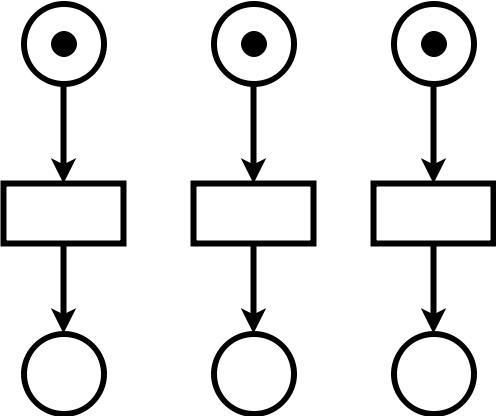
\includegraphics[width=1.2\linewidth,,keepaspectratio,right]{petrinet.jpg}
\end{figure}

\begin{figure}
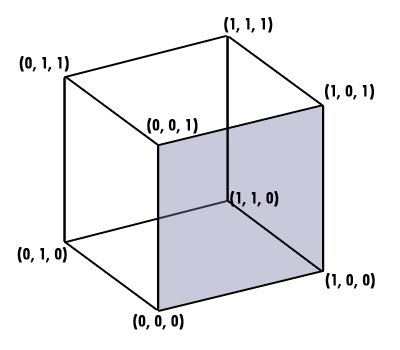
\includegraphics[width=1.5\linewidth,height=\textheight,keepaspectratio,right]{CubeVertices.jpg}
\end{figure}

\begin{figure}
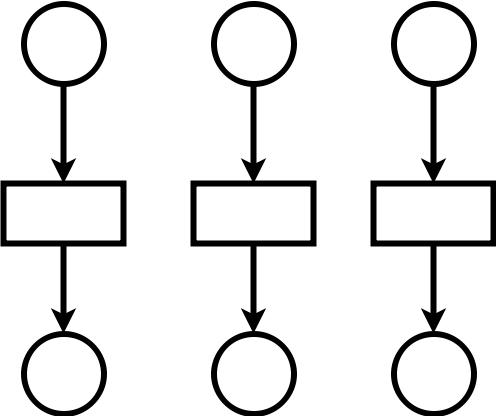
\includegraphics[width=1.2\linewidth,height=\textheight,keepaspectratio,right]{unfolding.jpg}
\end{figure}
\end{columns}
\end{frame}


%------------------------------------------------
\begin{frame}
\Huge{\centerline{The End}}
\end{frame}

%----------------------------------------------------------------------------------------

\end{document} 
